\chapter{Introduction}
\label{ch:intro}

\section{Churn in the telecommunication industry}

In recent years, the number of mobile phone users increased substantially,
reaching more than 3 billion users worldwide. The number of mobile phone service
subscriptions is above the number of residents in several countries, including
Belgium \parencite{itu2018itu}. Telecommunication companies are evolving in a
saturated market, where customers are exposed to competitive offers from many
other companies. \textcite{hadden2007computer} show that attracting new
customers can be up to six times more expensive than retaining existing ones.
This led companies to switch from a selling-oriented to a customer-oriented
marketing approach. By building customer relationship based on trustworthiness
and commitment, a telecommunication company can reduce the incentives for their
client to churn, therefore increasing benefits through the subsequent customer
lifetime value.

One of the various marketing processes used to improve customer relationship is
to conduct retention campaigns. This traditionally consists in selecting clients
according to some simple statistical criteria and offering them a promotion or
advantage. Typical promotions include a reduced invoice, free calls, SMS or data
volume. However, due to the limited nature of this statistical analysis, it is
plausible that the customers thus reached might never have planned to churn
in the first place. While this is of course not a problem for the customer, it
would be far more beneficial for the telecommunication company to be able to
focus the retention campaigns only on risky customers, in the hope of preventing
attrition that would otherwise occur if no action is taken. The problem of
detecting churn can be addressed with \emph{data mining}, by collecting data
about customers and using this information to infer typical patterns exhibited
by risky clients. This data-driven approach is nowadays taken by most major
telecommunication companies, and a part of the data mining literature is devoted
to churn detection. We will describe this approach further in the next section.



\section{Churn detection and prevention}

\begin{figure}[ht]
    \centering
    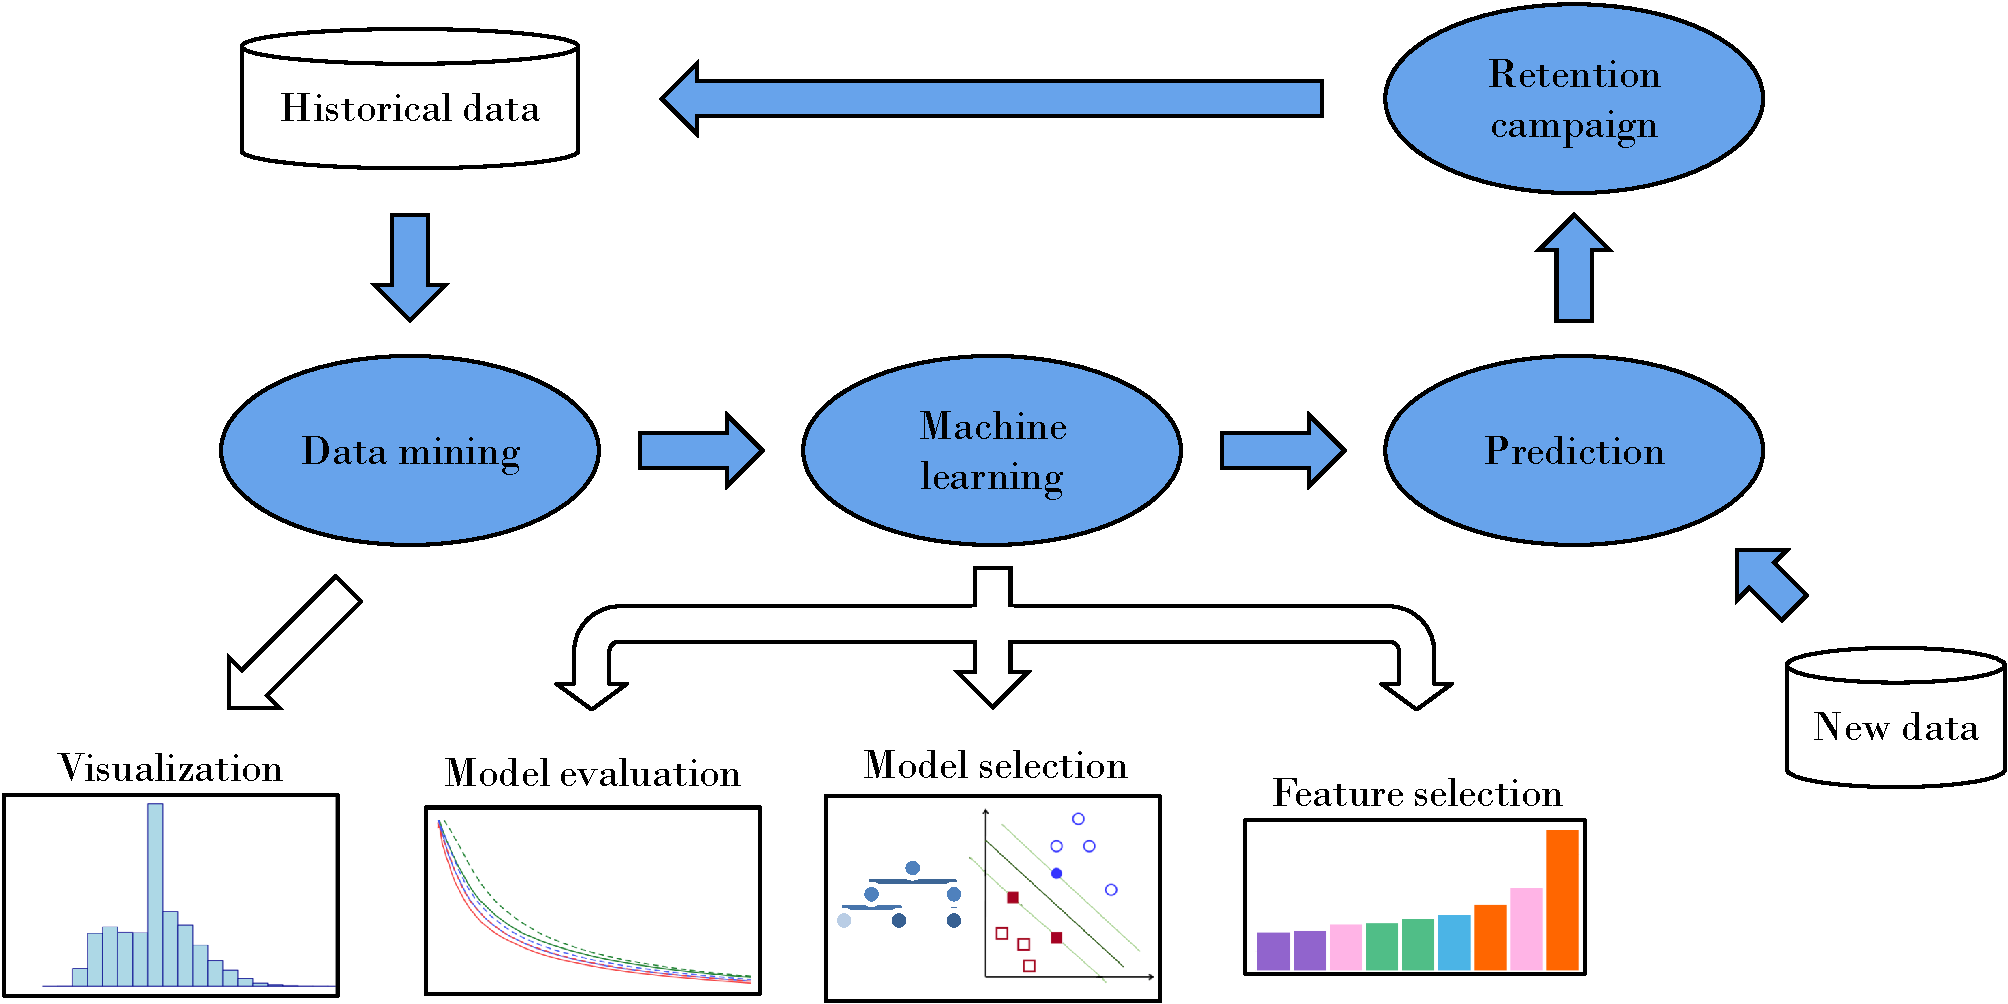
\includegraphics[width=\linewidth]{figures/churn_diagram}
    \caption{The churn prevention process implemented at Orange.}
    \label{churn_diagram}
\end{figure}

The churn prevention process (depicted in figure \ref{churn_diagram}) starts by
collecting data about the customers and creating a \emph{historical database}.
This data summarizes the calls, messages, internet usage and other actions
performed by the customers\footnote{This data is limited to the metadata of the
phone call, message, or internet usage. The content of the communication is
never used. Moreover, the location information in the metadata is also
excluded.}. It also includes information about the subscription, such as the
type of tariff plan, its price, the subscription date, and so on. Finally,
personal data provided by the customer may as well be used, such as the age or
the place of residence. \emph{Data mining} is then used on this database to
provide a quantitative understanding of the customers and their overall
behavior. In particular, the difference between churners and non-churners
behavior can be visualized. This is useful to decide which type of machine
learning procedure should be used for churn prediction, but can also bring
valuable knowledge to marketing and customer relationship teams. Once the data
is sufficiently understood, a set of relevant \emph{machine learning} models are
built. These models learn from the historical data the patterns typically
exhibited by clients that will churn in the near future. The types of patterns
being learned, the techniques used to find them, and the underlying assumptions
are dependent on the model under consideration. For example, a \emph{naive Bayes
classifier} assumes that each variable is independent of the others if we know
whether the customer is a churner or not. In order to decide which model should
be selected, the performances of each model are evaluated by testing them on
data left out of the training phase, and different models are compared. Feature
selection is also performed, and consists in evaluating the importance of each
variable for predicting churn and training the model by using only the most
important ones. This reduces the computation time and generally improves the
performances of the model since this reduces the noise unimportant variables
bring along. Once an efficient model has been selected, the latest customer data
is  submitted to the model which outputs a probability of churn for each
customer. By ordering the customers by churn probability, a list of the riskiest
customers is established and sent to the campaigning team. They split this set
of clients into a \emph{target group} and a \emph{control group}. Each customer
of the target group is offered an incentive either by phone call, email or
message, while the control group is left untouched. This allows, a few months
later, to evaluate the impact of the retention campaign by assessing the
difference of churn rate in retrospective in the two groups. Also, the accuracy
of the prediction model can be evaluated by comparing the control group and the
rest of the customer base

\section{Causal inference}

Depending on the resources available and the techniques used, this data mining
pipeline can successfully predict potential churners, therefore allowing to
conduct targeted retention campaigns. But campaigners are then faced with
another challenge: what should they propose to the selected customers? Indeed,
the predictions given by data mining algorithms usually just consist in a
probability of churn. This prediction therefore does not indicate \emph{why} the
customer is about to stop the subscription. We need different analysis tools to
tackle this problem. This is the purpose of \emph{causal inference}, which is a
formal approach to find the causes of some event in a system. Causal inference
is usually conducted through \emph{controlled randomized experiments}
\parencite{fisher1937design}. In the context of customer relationship
management, controlled experiments are possible through retention campaigns,
where the offers made to the customers act as variable manipulations. For
example, offering a discount would act on the variable ``invoice amount''. Such
an experiment is out of the scope of this master thesis since it requires time,
planning, and a collaboration with the direct marketing department. We thus
focus on data-driven approaches, which are based on some properties of the
statistical distribution of causally linked variable.

To give an example of how causal inference can be conducted without experiment,
consider the simplistic world where two types of phone are available, an
expensive one and a cheap one. The expensive phone type makes customers consume
more data per month than the cheap one because more data-hungry applications are
available on it. Also, it increases the probability of churn because these
phones are targeted more often by concurrent advertisement. We represent such
causal scenario with a \emph{directed acyclic graph} as in figure
\ref{fig:simple_causal}. We assume that once we know the phone type of a
customer, its data usage and its propensity to churn are independent, since
these are two different consequences of the customer's choice of phone. We
plotted the data usage against the probability of churn for each type of phone in
figure \ref{fig:simple_causal_plot}. A positive correlation can be observed
between data usage and churn but disappears when considering each phone type
separately. If a causal relationship also existed between data usage and churn
probability, the statistical dependency would still be visible, even when
conditioning on the phone type. This idea of conditioning to discard putative
causal links is at the basis of most causal inference algorithms.

Such inference methods are based on a number of modeling assumptions, such as
the ability to represent the underlying causal mechanism by a graph as in figure
\ref{fig:simple_causal}, or the absence of confounding factor. This latter
assumption would be violated if, in our previous example, the age of the
customer influences both its choice of phone type and its propensity  to churn.
The causal inference algorithm would still conclude that the expensive phones
cause clients to churn, while in reality, they churn solely because of their
young age. This sort of erroneous conclusions can lead to ineffective action in
retention campaigns. Other inference methods imply other assumptions, and care
must be exercised when using them.

\begin{figure}
    \centering
    \begin{tikzpicture}
        \begin{scope}[every node/.style={ellipse,thick,draw}]
            \node (1) at (0, 0) {Phone type};
            \node[below left = of 1] (2) {Data usage};
            \node[below right = of 1] (3) {Churn};
        \end{scope}
        \begin{scope}[>={Stealth[black]},
            every edge/.style={draw=black,very thick}]
            \path [->] (1) edge node {} (3);
            \path [->] (1) edge node {} (2);
        \end{scope}
    \end{tikzpicture}
    \caption{Toy example of a causal diagram.}
    \label{fig:simple_causal}
\end{figure}

\begin{figure}
    \centering
    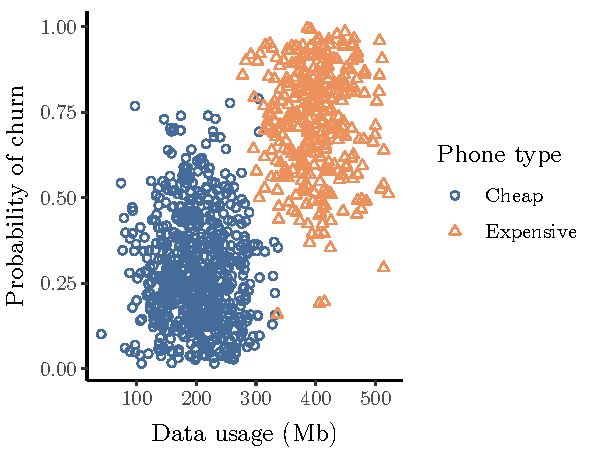
\includegraphics[width=4in]{figures/simple_causal_plot.pdf}
    \caption{Toy example of data usage against the probability of churn for
    different phone types.}
    \label{fig:simple_causal_plot}
\end{figure}

\section{Context and motivation}

This master thesis is conducted in collaboration with Orange Belgium, and
originated from the long-lasting scientific collaboration between Prof. Gianluca
Bontempi (ULB Machine Learning Group) and Dr. Olivier Caelen (Orange Belgium).
This collaboration enables us to work on real-world data, in Orange
premises, and with people directly involved in the subject (data science and
business intelligence teams at Orange). The churn prediction problem is
challenging in many regards: the dataset is large (in our case, 1.5 million
entries per month, over 5 months), highly imbalanced (there are very few
churners in the whole customer base), and highly overlapping (many non-churners
exhibit the same behavior as churners). It is therefore an interesting subject
for a master thesis in machine learning, since it requires the use of different
state-of-the-art tools for overcoming these challenges.

The churn prediction task shares many similarities with the fraud detection
problem, for example regarding the class imbalance and overlap, and the large
amount of data. The Machine Learning Group (MLG) has a fruitful collaboration
with Wordline in fraud detection since 2012 when Prof. Bontempi wrote and
supervised the Doctiris project ``Adaptive real-time machine learning for credit
card fraud detection'' (PhD student: Andrea Dal Pozzolo). The research activity
in this domain continued thanks to ``Brufence: Scalable machine learning for
automating defense system'' project and the recent TEAM-UP project DefeatFRAUD.
This thorough experience in the subject is a motivation and a valuable asset to
pursue research in churn prediction.

The interest for causal inference comes from the experience of the MLG in the
subject. They mainly applied causal inference onto bioinformatics application,
such as gene selection \parencite{bontempi2011multiple} or microarray data
\parencite{bontempi2010causal}. More recently, a competition on causal analysis
was organized on the Kaggle website
(\url{https://www.kaggle.com/c/cause-effect-pairs}), with the goal of fostering
causal discovery between two variables. This led to the development of new
methods, notably using machine learning \parencite{bontempi2015dependency}.
Moreover, the use of causal inference is seldom explored in the literature on
churn prevention. It is thus stimulating to conduct research at the intersection
of these two domains, benefiting from the technical expertise of the MLG and
the business knowledge of Orange.

\section{Contributions}
The main contributions of this thesis are
\begin{itemize}
    \item Understanding of the churn prediction problem with a real-world
    dataset from a telecom company (section \ref{sec:churn_data}).
    \item Evaluation of the predictive power of a state-of-the-art churn
    prediction model, and the impact of several variations of the model by using
    different features and different type of subscription contracts (section
    \ref{sec:churn_exp}).
    \item Assessment of the directionality of the impact of a variable on
    prediction, by shifting the value of the variable in the test set and
    measuring the difference in average predicted score (section
    \ref{sec:churn_sens}).
    \item Study of causal analysis, and its application to churn prediction from
    observational data (section \ref{sec:causal_experiments}).
\end{itemize}

\section{Outline}

This master thesis is partitioned into 5 chapters, presented here.

\begin{enumerate}
	\item (Chapter 1) An introduction to the problem of churn in the
	telecommunication industry, the current methods in use to tackle it, and the
	contributions of this master thesis.

    \item (Chapter 2) Exposition of the state of the art in churn prediction
    and causal analysis.
    \begin{itemize}
        \item Churn prediction: choice of predictive model, data preprocessing,
        class balancing and evaluation measure.
        \item Causal analysis: Bayesian network learning, Markov blanket
        inference, information-theoretic filters, bivariate and supervised
        methods.
    \end{itemize}

	\item (Chapter 3) Assessment of a churn prediction model on Orange customer
	data. This chapter is further divided into:
	\begin{itemize}
		\item Presentation of the dataset
		\item Description of the data preparation
		\item Description of the experimental setting
		\item Presentation of the results
        \item Comparison to other state-of-the-art methods
		\item Conclusion and main outcomes of the experiments
	\end{itemize}

    \item (Chapter 4) Exploration of causal inference methods for churn
    prevention:
    \begin{itemize}
        \item Theoretical background for causal inference
        \item Scope of application
        \item Prior knowledge of the possible causes of churn
        \item Description of the experimental setting
        \item Presentation of the results
        \item Discussion and conclusion
    \end{itemize}

    \item (Chapter 5) A conclusion, divided into the following topics:
    \begin{itemize}
        \item Summary of our results
        \item Discussion of potential threats to the validity of our results
        \item Explanation of the added value of this thesis for Orange Belgium
        \item Presentation of planned future work
        \item Final conclusion
    \end{itemize}
\end{enumerate}

\section{Notation}

The mathematical notation used throughout this document is presented in table
\ref{tab:notation}. Bold font denotes vectors or sets, and uppercase letters
denote random variables. An uppercase bold font thus denotes a set or vector of
random variables.

\begin{table}[h]
    \centering
    \begin{tabular}{ll}
        \toprule
        $n$ & Number of features\\
        $\mathcal X\subseteq\mathbb R^n$ & Feature space\\
        $\bm X = [X_1,\dots,X_n]$ & Vector of random variables in $\mathcal X$\\
        $\bm x = [x_1,\dots,x_n]$ & Feature vector, realization of $\bm X$\\
        $\mathcal Y=\{0, 1\}$ & Target label space\\
        $y\in\mathcal Y$ & Example label \\
        $P(e)$ & Probability of an event $e$\\
        $S$ & Random variable of predicted score as a function of $\bm X$\\
        $s$ & Predicted score for a given $\bm x$, realization of $S$\\
        $t\in [0, 1]$ & decision threshold\\
        $f_y(s)$ & Probability density function of $S$ for instances labeled $y$\\
        $F_y(s)$ & Cumulative distribution function of $S$ for instances labeled $y$\\
        $X\perp Y$ & Random variables $X$ and $Y$ are independent\\
        $\bm X\setminus \bm Y$ & Set difference between $\bm Y$ and $\bm Y$\\
        \bottomrule
    \end{tabular}
    \caption{Summary of the mathematical notation.}
    \label{tab:notation}
\end{table}
